\section{Introduction} \label{sect:intro}

You and the person next to you might not be using the same Internet. With
ever increasing diversity and interlinking of online services  --- content distribution networks, cloud computing, CDN brokers,
cloud brokers, ad brokers, load balancing, user tracking, geoIP, and more --- even the
implications
of loading a single web page are no longer straightforoard \cite{butkiewicz2011}. Often, failure to
recognize the whole as distinct from the sum of its parts has inhibited progress
and hampered performance in networking technology \cite{blair15iwarm,kakhki2017taking}. In the same way a city's
skyline cannot be anticipated by the artitect of a single  building, the
``digital skyline'' of the Internet can be neither predicted nor fully
controlled by any single entity.
However, skylines can always be \emph{observed}.

Even across a single network service, client experiences may diverge. In Figure
\ref{fig:dnsmiss}, we provide a high level illustration of how this can happen.
In subfigure \ref{fig:dns},  a client intending to connect to example.com submits a DNS query. We do not
show the minute details of
the DNS resolution process, which is itself multi-tierd and possibly involving
cooperation from many separate stakeholders. What is important to know is that
eventually, the client's request reaches the nameserver responsible for
example.com. The nameserver uses what is often internal, proprietary
logic to decide which of example.com's network resources the client should be
connected to. In subfigure \ref{fig:mismatch}, we are reminded that this client
is not the only one from its subnetwork to access example.com. However, as illustrated,
the client's peers may not necessarily be directed to the same content resource, despite
having carried out essentially the same DNS resolution process and possibly
sharing the same edge network. This potential for mismatch between clients only
grows as the number of domains considered increases --- which it will, often on
a single web page.

In this project, we explore the complex combination of independently operating
resource allocation schemes and assess their behavior in \emph{aggregate}. To
enable our research, we introduce a new similarity measure, common network
resource exposure (CNRE), which captures the extent to which a pair of clients
are directed to the same network targets as each other across a broad set of
domains. CNRE is, to our knowledge, the first ever method to quantify
cross-provider DNS redirection patterns and their collective behavior. 

We test and assess CNRE using 302 web content hosting domains for each CNRE
calculation.  To do this, we collect latency and DNS measurements for each
domain from each of 9,024 globally distributed clients and perform over 40
million pairwise CNRE calculations between them. Our experiments 
validate common network research exposure as a useful measure and explore its
relationship with other client properties.

\begin{figure*}
    \center
        \mbox{
            \begin{subfigure}[b]{0.5\linewidth}
                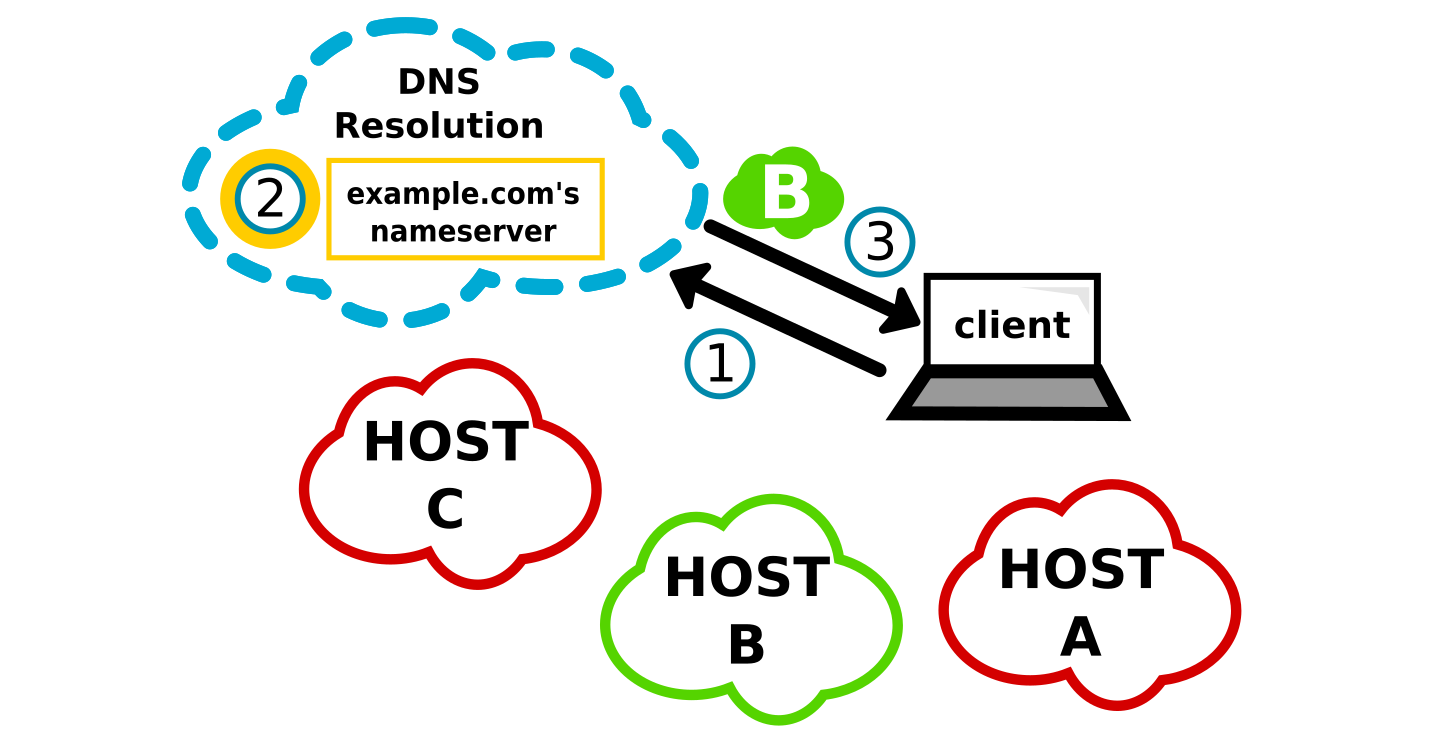
\epsfig{file=figs/dns_resolution.png, width=1\linewidth}
                \caption{\label{fig:dns}}
            \end{subfigure}
            \begin{subfigure}[b]{0.5\linewidth}
                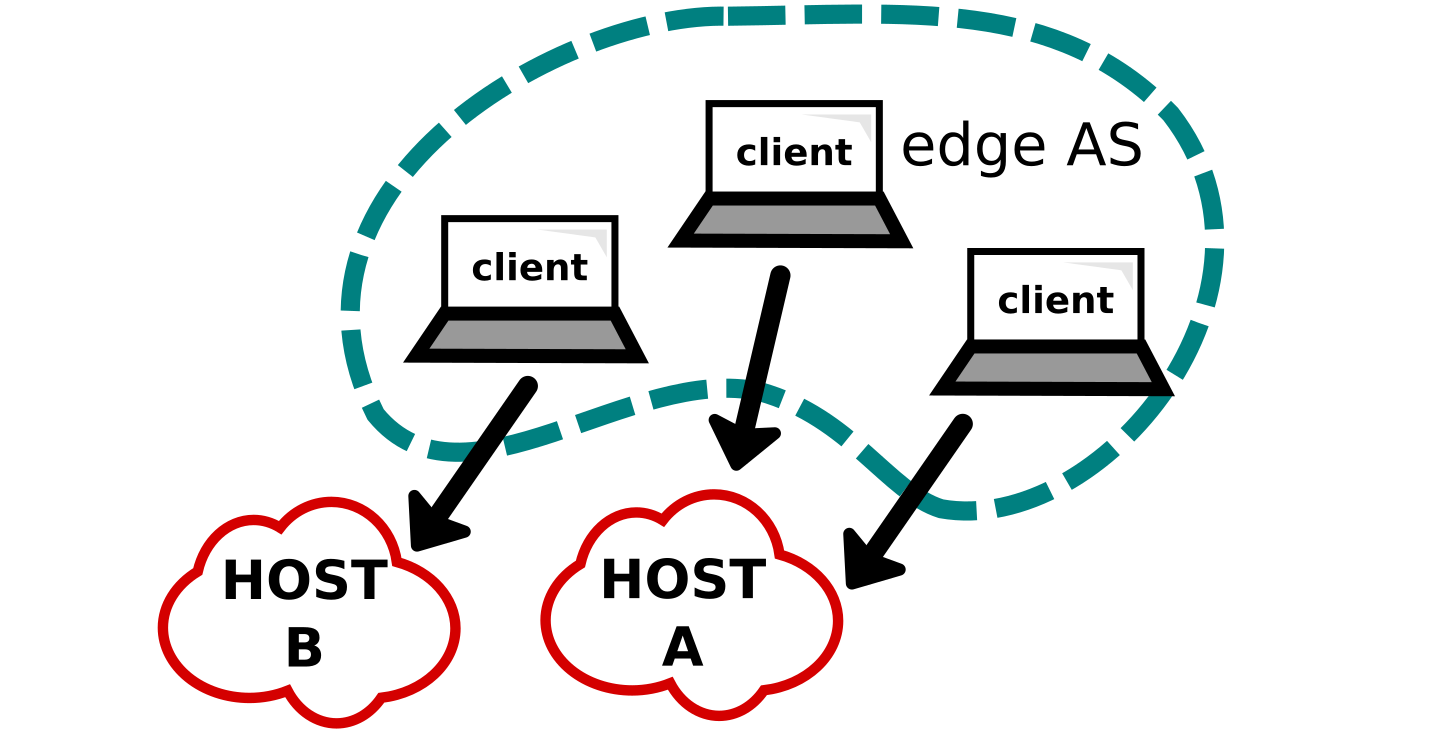
\epsfig{file=figs/client_mapping.png, width=1\linewidth}
                \caption{\label{fig:mismatch}}
            \end{subfigure}
        }
    \caption{
        Illustration of network resource allocation. Figure \ref{fig:dns} shows DNS resolution at a high level: 1)~The client deploys a DNS query for example.com. 2) This query ultimately reaches nameserver responsible for example.com and decides which of example.com's network resources should serve the client. 3) The nameserver's resource selection is returned to the client. Figure \ref{fig:mismatch} shows an example of how clients with similarly described locations may
        be directed to distinct network resources.
    }
    \label{fig:dnsmiss}
\end{figure*}

In order to understand CNRE, we performed an exhaustive set of measurements to frame
client experience on a per \emph{site} basis, as opposed to per individual domain. In this work, we capture a
snapshot of both DNS resolutions and latency measurements toward the 304 domains that appeared most
frequently in the top 2441 most popular webpages. Our measurements span over
9,000 unique
clients spread across 185 countries and 3637 autonomous systems. We performed over 52 million pairwise
comparisons with the results of these measurements to explore the patterns and implications of common network resource exposure. 

This project makes the following contributions: 

\begin{itemize}%\parskip0pt \parsep0pt
    \item We perform a large scale exploration of client network performance on a per webpage level. Our
        raw results are publicly available on the RIPE Atlas platform.
    \item We introduce the common network resource exposure (CNRE) similarity
        measure, which quantifies the extent to which clients are directed to
        the same set of web resources.
    \item  We quantify the degree of alignment between conventional grouping schemes (country, ASN, and BGP prefix)
        and CNRE.
    \item We identify clusters of clients that share especially high levels of
        common network resource exposure and analyze their properties.
    \item We approximate the effective geographic ``centers'' of CNRE clusters,
        where their target network resources are most likely concentrated.
\end{itemize}

% RELATED WORK and PROBLEM FRAMING
\section{Problem Space} \label{skyspace}

In this paper, we aim to quantify the degree of overlap in the sets of network
resources (\emph{i.e.} servers) that different clients are exposed to when
browsing the same websites. We further aim to assess the implications of this
overlap and derive the effective aggregated hubs of these resource sets. This endeavor is chiefly motivated by two key
observations. First, it is well documented that web services rarely operate in
isolation, but rather in (potentially large) combinations. Past work found that the
majority of popular websites: 1) point to web content stemming from \emph{at least}
7 distinct origins~\cite{butkiewicz2011} and 2) trigger upwards of 50 DNS
resolutions for a single client~\cite{dnssly}. Second, as discussed in
Section \ref{sect:intro} and illustrated by Figure \ref{fig:dnsmiss}, it is well
established that DNS answers often vary across clients, even for a single domain
\cite{ecs15sigcomm,Calder2013,benchaita2016stability,exploringedns,warrior2017drongo}.
Below, we detail the anticipated applications for this work and discuss related
research to provide the reader with necessary context through which the rest of
this paper can be understood.

\subsection{Applicability} \label{applicability}

This work's most direct and immediate use case lies in influencing client
selection in large scale Internet measurements. For researchers, likely unaware of the relatively
hidden allocation schemes of the wide array of CDN platforms and other large content distributors,
it is difficult to determine, a priori, the degree of similarity between clients. Knowledge of
whether there is a high probability that a pair of clients are being directed to altogether
different resources may be significant to their experiment design. This approach to experiment
design is in line with RIPE Atlas, one of the largest client based measurement platforms,
which maintains
an exhaustive set of tags on all of their clients in order to help researchers and network operators
filter and refine the set selected for their experiment \cite{ripe-atlas}. Further, more abstract
applications may include, but are not limited to, distributed denial of service mitigation
\cite{anycastvsddos} and CDN node deployment \cite{35590, Tariq}.

In addition to the above applications in currently existing paradigms, we also
speculate a significant potential use case for the techniques discussed in this
paper. For a variety of reasons --- most notably, security concerns ---
providers (\emph{i.e.} CDNs and other content hosting platforms) often deem it
within their best interest to limit public visibility into the details of the
respective platform's infrastructure and implementation scheme (\emph{e.g.} the
exact locations, IP ranges, or client mappings of all of their servers or
datacenters). The approach and findings presented Section \ref{sect:analysis}
offer a means to effectively capture the \emph{properties} --- geographic
resource locations, number of resource locations, performance, etc --- of these
providers while \emph{obfuscating} the specifics of any individual provider
behind aggregated hubs we refer to as geographic ``centers''. In other
words, our approach may offer the opportunity for openness and collaboration in a
space that is otherwise kept deliberately opaque.

\subsection{Related Work} \label{related}

The most similar body of related work involves anycast CDN catchment analysis, which aims to
investigate the set of clients routed towards particular CDN points of presence (PoPs)
\cite{anycast, anycastvsddos, vdmscatchment}. Our work differs significantly in scope: to our 
knowledge, we are the first to investigate what we refer to as \emph{aggregate catchments}, the joint
behavior of many anycast CDN catchments as well as unicast CDN targets, spread across many content
distribution platforms. Conversely, this related body work either focuses on individual platforms or
specific services \cite{anycast, anycastvsddos, vdmscatchment}. 

Several authors have attempted to discover the topology of large CDN platforms through large scale
measurement studies \cite{webcart, Calder2013, benson11}. While their findings are potentially of
use in this project, their goals and contributions run parallel to what we aim to accomplish. They
seek to identify the properties and locations of CDN resources; conversely, we seek to identify the
target pools (sets of clients) of overlapping CDN resource catchments \cite{webcart, Calder2013,
benson11}. Other work close to this space investigates the performance of a particular CDN
deployment scheme \cite{ecs15sigcomm}.

To our knowledge, no existing body of work has attempted to quantify the extent
to which clients are exposed to the same web resources across domains.  However,
work concerning security in internationally networked platforms do take network
resource exposure into account. For example, some work has identified scenarios
where traffic routed through certain neighboring countries is sometimes censored
or manipulated by middleboxes in the transit country \cite{Anonymous:2012}. To the same end, the
authors of \cite{Edmundson:2016} developed a means to guarantee traffic is not exposed to
specific territories. In a similar light, many globally distributed platforms
employ ``geoblocking'' to restrict content access to particular regions \cite{McDonald:2018}. As
a new way to quantify resource exposure in general, our work runs parallel to and may
be of use to these areas of study.
